\section{Method}
\label{sec:method}

\begin{figure}[t]
\centering
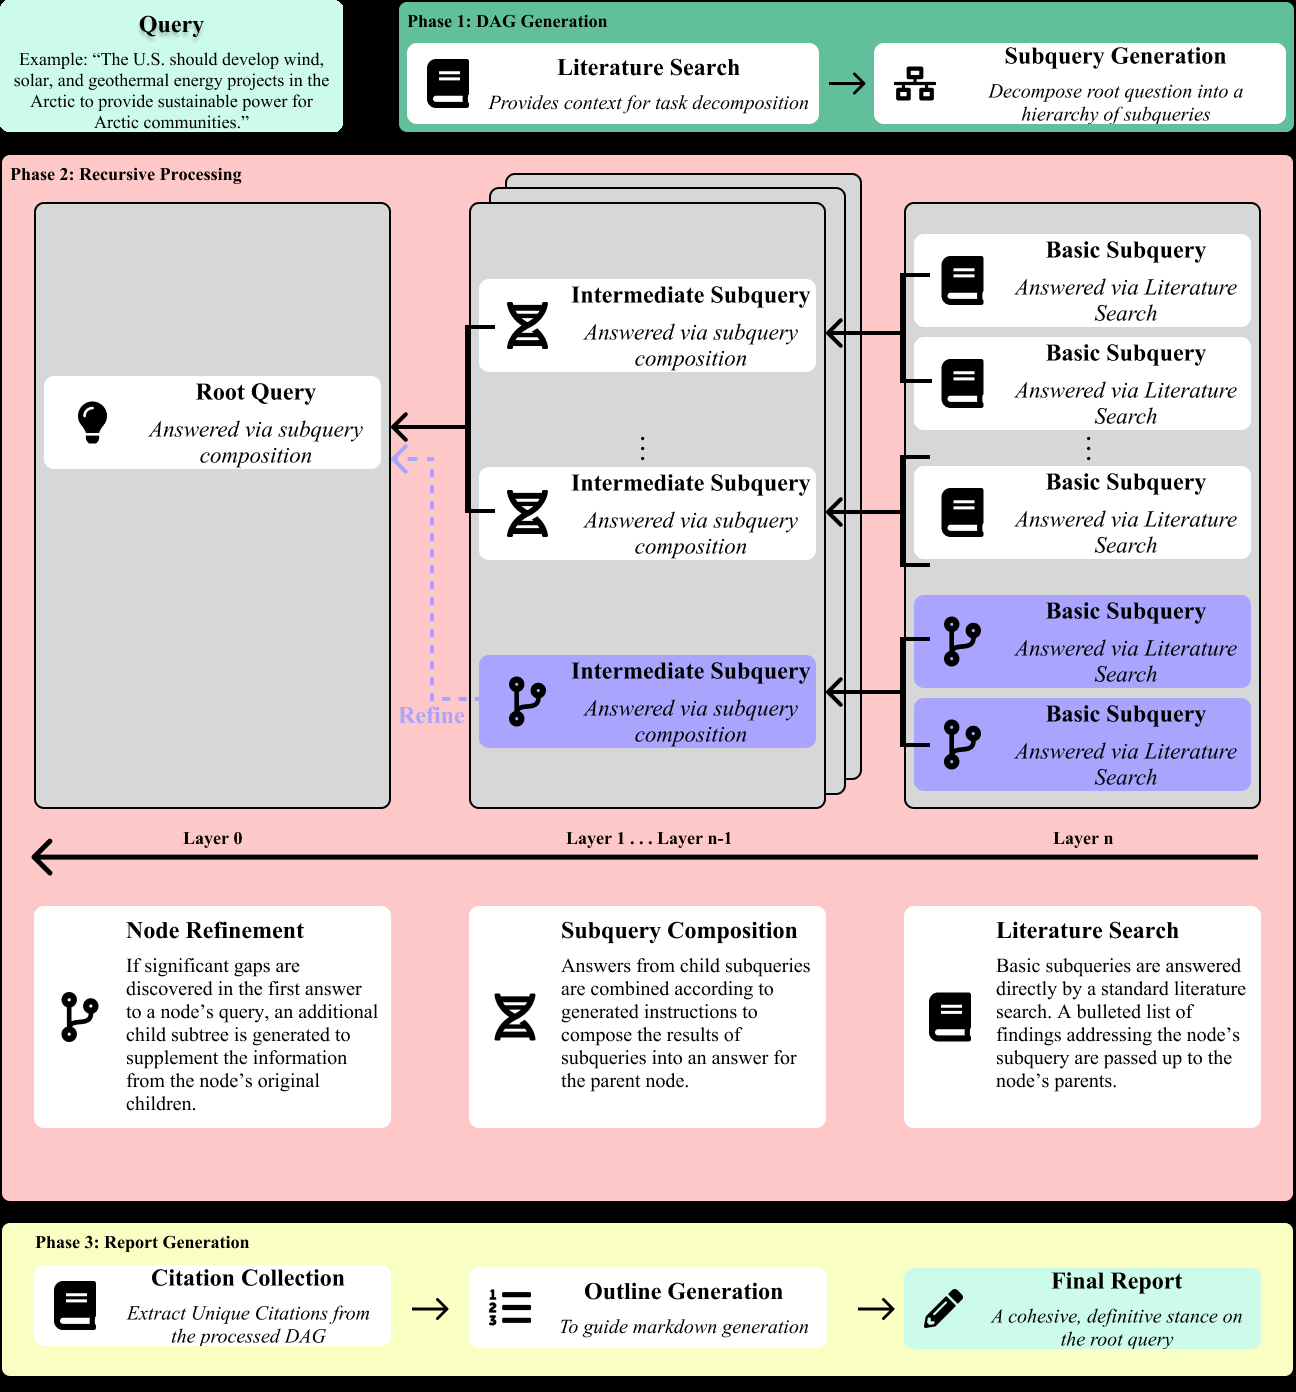
\includegraphics[width=\linewidth]{figs/pipeline.png}
\caption{The three phases of \sys{}. A literature search gives context for decomposing the query into a DAG of sub-queries (Phase 1). Leaves are answered by literature search, parents are composed from their children, and nodes with gaps are refined with new sub-trees (Phase 2). The answered DAG is turned into an outline and a report that argues the root answer (Phase 3).}
\label{fig:pipeline}
\end{figure}

\sys{} takes a research question and returns a report that argues an answer to it, with inline citations to web sources. It runs in three phases: DAG generation, recursive processing, and report generation. This section describes the pipeline as it was when the reports in \Cref{sec:experiments} were generated; \Cref{app:changes} describes the code versions involved and how the released code differs. Every language-model call is a DSPy signature \citep{khattab2024dspy}, reproduced in \Cref{app:prompts}.

\paragraph{Literature search.}
Both the planning phase and the leaf nodes use the same literature-search routine. A planning model turns a question into web queries, a retriever fetches results through the Serper API, scrapes the pages, embeds the passages with \texttt{text-embedding-3-large}, and keeps the passages closest to the query, and an answer model writes a cited answer from them. A completeness check decides whether to search again, up to a fixed number of retriever calls per question.

\paragraph{Phase 1: DAG generation.}
A short literature search on the root question gives the planner context. The planner then builds the DAG layer by layer. For each node in the current layer it generates child sub-questions, conditioned on the node's question, the literature summary, the children generated so far, and the structure of the whole DAG, so that siblings do not overlap and the children together answer the parent. The depth of the DAG, the total number of nodes, and the number of children per node are capped. A second pass writes composition instructions for every parent: given the parent's question and expected answer format and its children's questions, the model states how the children's answers combine into the parent's. The instructions reference children by their identifiers, so the dependency is explicit and can be checked later.

\paragraph{Phase 2: recursive processing.}
The DAG is sorted topologically and processed from the leaves to the root. Leaves are answered in parallel by literature search; the answer model writes bullet points in the node's expected format and keeps every citation from the search. Parents are composed in sequence: the children's answers, the composition instructions, and the expected format go to a synthesis model that may use only the children's content, must cite by the children's citation numbers, and must say so when children contradict each other. Citations are deduplicated as they pass up the graph.

A composed answer can still miss something the plan did not anticipate. After composing a parent, a gap explorer lists possible gaps in the answer, and a gap evaluator judges, at a configurable level of conservatism, whether any of them matters enough to act on. If so, the pipeline generates a sub-tree of new sub-questions for the gaps, attaches it under the parent, processes it like the rest of the DAG, and recomposes the parent. Each parent is refined at most once in the released configuration.

\paragraph{Phase 3: report generation.}
The answered DAG is serialized as text and its citations are collected into one numbered list. An outline model, instructed to argue a stance on the root question, writes an outline whose sections follow the hierarchy of the DAG. A report model then writes the report from the outline and the DAG, keeping the citations, taking the stance of the root answer, and titling the report with the claim rather than the question. Citation numbers are normalized and a bibliography is appended.

\begin{algorithm}[t]
\caption{\sys{}}
\label{alg:pipeline}
\begin{algorithmic}[1]
\Require motion $m$; limits on depth $d$, nodes $n$, children $c$; refinement rounds $\rho$
\State $L \gets \textsc{LiteratureSearch}(m)$ \Comment{context for planning}
\State $G \gets$ root $r$ with $q_r = m$
\For{each layer $\ell = 0, \dots, d-1$} \Comment{Phase 1}
  \For{each node $u$ at depth $\ell$}
    \State add children $\textsc{PlanChildren}(q_u, L, G, c)$ under $u$, within the node limit $n$
  \EndFor
\EndFor
\For{each parent $u$} $\kappa_u \gets \textsc{CompositionInstructions}(q_u, \{q_v : v \in C(u)\})$ \EndFor
\For{each node $u$ in topological order, leaves first} \Comment{Phase 2}
  \If{$u$ is a leaf}
    \State $(a_u, S_u) \gets \textsc{AnswerFromSearch}(q_u)$
  \Else
    \For{$k = 0, \dots, \rho$}
      \State $a_u \gets \textsc{Compose}(q_u, \{a_v\}_{v \in C(u)}, \kappa_u)$; \quad $S_u \gets \bigcup_{v \in C(u)} S_v$
      \State $\Delta \gets \textsc{FindGaps}(q_u, a_u)$
      \If{$k = \rho$ \textbf{or} $\Delta = \emptyset$} \textbf{break} \EndIf
      \State attach a sub-tree for $\Delta$ under $u$ and process it as in Phase 2
    \EndFor
  \EndIf
\EndFor
\State $O \gets \textsc{Outline}(m, a_r, G)$; \quad $R \gets \textsc{Report}(O, m, a_r, G)$ \Comment{Phase 3}
\State \Return $R$ with a bibliography of $\bigcup_v S_v$
\end{algorithmic}
\end{algorithm}

\paragraph{Cost.}
Let $|V_\text{leaf}|$ and $|V_\text{par}|$ be the numbers of leaves and parents after refinement. Each leaf costs one literature search, which is at least one query-generation call, one retrieval with embedding, one answer call, and one completeness check. Each parent costs one composition call per round and one gap check. Planning adds one call per parent for children and one for instructions, and writing adds two. The number of model calls is therefore about $4|V_\text{leaf}| + (3 + 2\rho)|V_\text{par}| + 3$, linear in the size of the graph, and leaves can be processed in parallel. The logged run in \Cref{app:dag} has \dagLeaves{} leaves and \dagParents{} parents, so it makes on the order of 40 model calls, compared with one or a few for a single-pass report.

\paragraph{Models and limits.}
The evaluation runs used GPT-4.1-mini for retrieval-side answer generation and planning, GPT-5 for DAG generation, synthesis, and report writing, and \texttt{text-embedding-3-large} for retrieval, all through Azure OpenAI; the released code also runs on the OpenAI API. The released defaults cap the DAG at depth 2, 50 nodes, and 10 children per node, with one retriever call per literature search and one refinement per parent.
